\chapter{Write Away 7}

\begin{figure}[H]
    \centering
    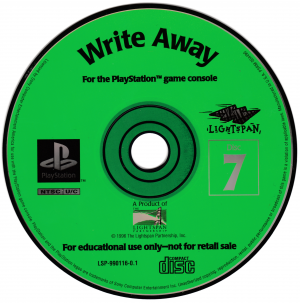
\includegraphics[width=\textwidth/2]{./Games/WriteAway/Images/WriteAway7CD.png}
    \caption{Write Away 7 CD}
\end{figure}

The seventh of the ten Write Away games published and released by The Lightspan Partnership for the PlayStation 1.

Write Away 7 features ten video programs, including an introduction video, eight story videos, and a conclusion video:

\begin{itemize}
    \item Write Away Episode Seven Introduction
    \item The Boy Left Out by Jack Lee
    \item Name Poem by Samir Hussain
    \item A Treasure Hunt by Carley Moore \& Abby Mathis
    \item The Day President Clinton Came to Our School by Sara Milton
    \item Alice in Halloween Land by Jasmine Khan \& Hugh Kennedy
    \item A Whale Speaks by William Burke
    \item Dreaming on Skates by Darla Garcia
    \item Dangerous Surfing Veggies by Michael Clayton
    \item Write Away Conclusion
\end{itemize}

\clearpage
\newpage

\section{Transcriptions}

\subsection{The Boy Left Out by Jack Lee}

NEWSPAPER ANNOUNCER (VOICE OVER):
Extra, extra!
Read all about it!
Oregon boy says they laughed when I wanted to play!
Third-grader Jack Lee from Eugene, Oregon, tells us all about it in his story The Boy Left Out.

NARRATOR:
This is the story of a kid named John.
John was an unhappy boy because he always got left out of team sports at school.

OSCAR:
All right, everybody, we're here now.
We can choose up sides to play a little tag football.

EVERYONE:
Yeah!

JOHN:
Oscar!
Oscar!
Oscar!
Can anybody play?

OSCAR:
Uh...
We'll see.
You pick first.

GIRL 1:
I pick Jim!

OSCAR:
Okay, I pick, uh, Sally!

SALLY:
Yeah!

GIRL 1:
Well, that takes care of everyone who really can play football.

SALLY:
Oh, here John, here.
Here's some money.
You go and buy us some sodas.

JIM:
Yeah, and if you're really lucky, maybe we'll let you cheerlead for us.

SALLY:
Hahaha!

OSCAR:
Come on, guys, let's go.

JOHN:
They may be laughing at me now, but someday, as Joe Montana is my witness, I will play football.

NARRATOR:
John never got picked to play sports, but he didn't give up.
Then one day, John's big chance came.
Jim was hurt, and the team was one man short.

OSCAR:
Well, Jim's out.
Looks like you'll have to forfeit because you don't have another player.
Hahaha!

JOHN:
Let me play!
Let me play!
Please, look, look, me me me, hello!
Please please please please please!

GIRL 1:
Oh, I guess I'll have to take John.
Okay, John, you better be good or else.

JOHN:
Don't worry, just passing that pigskin!
Yay!

OSCAR:
Wow, John, you were wonderful!
From now on, I'm always putting you on my team.

GIRL 1:
No way!
My team!

OSCAR:
No, my team!

NARRATOR:
Yes!
John could play football!
But one day, the game changed to baseball, and with that went John's luck.

SALLY:
Strike three.
You're out!

OSCAR:
Boy, John, you really stink at this game.
I think you should stick to football.

JOHN:
You're right.
I will stick to football.
And I'm gonna practice every day.
I'm gonna lift weights, I'm gonna eat right, and I'm not gonna go out with girls on school nights.
Sorry.
And I'm gonna get really good grades because when I grow up, I'm gonna be in the NFL!

NARRATOR:
And now John does play in the NFL as a wide receiver.

NFL MANAGER:
Oh, if I had nine more like him, I could rule the world!

CHEERLEADER:
Yaay John!

JOHN:
I've learned a valuable lesson.
If you have a dream, never, ever give up.
Just keep on trying.

\subsection{Name Poem by Samir Hussain}

NEWSPAPER ANNOUNCER (VOICE OVER):
Extra, extra!
New poet discovered in New Jersey!
Fifth-grader Samir Hussain shares a poem based on his name, in 'Name Poem.'

BOY:
Smart in sports, and smart in school.

GIRL:
Also cool!

BOY:
Well, maybe sometimes I'm a fool.
Well hockey I can play, understand what people say.

HOCKEY PLAYER:
Go get 'em!

BOY:
Sneaky I am not.
Yeah!
Sometimes people like me a lot.
Aiming for a good life, I am always nice.

MAN:
Ouch!

BOY:
And never will I play with a knife.
'Name Poem,' The End.

\subsection{A Treasure Hunt by Carley Moore \& Abby Mathis}

NEWSPAPER ANNOUNCER (VOICE OVER):
Read all about it!
Pirate saves beautiful princess.
Take a trip with kindergartner Carley Moore and fourth-grader Abby Mathis from Alps Road School in Athens, Georgia, as they go on a treasure hunt.

SCOUT (VOICE OVER):
Once long ago, there lived a pirate, a mean pirate who hated all around him.
He only loved one thing - his pet parrot.

CAPTAIN:
Oh, me beautiful bird, why won't you eat?
You haven't spoken for two days.
You're the only thing here I love in this whole world.
That is, except for me treasure!

SCOUT (VOICE OVER):
Now, on this ship, there were also two very good pirates who took care of the mean pirate.

PIRATE 1:
Arr, I'm all done swabbing the deck.
And if I say so myself, this deck is so shiny I can almost see myself in it!

PIRATE 2:
Arr!
And I'm done peeling these potatoes for the wonderful shepherd's pie I'm baking for dinner.
But I'm worried about the captain - he keeps trying to feed his parrot.

PIRATE 1:
Aye.

PIRATE 2:
Maybe one of us should break the news to him that we think Polly left this world a week ago.

PIRATE 1, PIRATE 2:
Nah.

SCOUT (VOICE OVER):
They sailed on and on until one day, when the mean pirate came up with a plan.

CAPTAIN:
Arr, I've got to hide me treasure so that no one will find it, and then I'll claim it later.
What's this I see?
Why, it's an island!
Well, get me treasure, and we'll bury it on that island.
Let's get in the rowboat, let's go!

SCOUT (VOICE OVER):
The mean pirate was gone, and soon the good pirates realized this.

PIRATE 2:
You know, it seems awfully quiet around here.

PIRATE 1:
Aye, I wonder, where's the captain?
Look, there he goes on that island to bury the treasure.
The treasure that we helped him get.

PIRATE 2:
Aar, how rude.
Let's swim to the island, find the treasure, and take what rightfully belongs to us.

PIRATE 1:
Aar.

PIRATE 2:
But we'll let him keep the parrot.

SCOUT (VOICE OVER):
The mean pirate took the treasure and went to hide it.
Meanwhile, the two nice pirates were in pursuit.

PIRATE 2:
Arr, I see him.
He went through the bushes, up the mountain, swam through the lake, and he's now burying the treasure on the other side of the island.

PIRATE 1:
Arr, you have excellent eyesight.

PIRATE 2:
Why, thank you.
Let's go.

SCOUT (VOICE OVER):
The mean pirate was about to bury his treasure when he heard a female voice cry out.

PRINCESS:
Help!
Help!
I am the princess of this island, and I've been trapped on this hill for so long!
Won't you help me down?

CAPTAIN:
No, I don't have time to help you.
I've got to hide me treasure.
Don't worry, Polly, she means nothing to me.
You're the only one I've ever loved.
    [Now, we'll] bury this treasure, and we'll be done with it.

PRINCESS:
Help!
Help!
I am the princess of this island, and I've been stranded on this hill for so long.

PIRATE 2:
Don't worry lassie, we'll help you.

PIRATE 1:
Here, let me help you down.

PRINCESS:
Thank you, you're both so brave and kind!
How can I reward you?

PIRATE 2:
Have you seen a mean pirate here with a treasure?

PRINCESS:
Ah, and a parrot that looks like it's sleeping on his shoulder that he talks to?
Why yes!
He went that way.
Let me show you.

SCOUT (VOICE OVER):
But just as the three were about to leave, the earth shook and rocks came falling down on them and buried them.

PIRATE 2:
The mean pirate must have made this avalanche to try to stop us.

PIRATE 1:
Hey, but he failed.
When he started the avalanche, the treasure must have fallen out of his hands because here he is.

PIRATE 2:
Arr.

PIRATE 1:
But where's the princess?

SCOUT (VOICE OVER):
The mean pirate had pulled the princess out of the rubble and kidnapped her.

CAPTAIN:
Oh they'll be back to try to save you, but I'll stop them and I'll get me treasure back.
And now, to take a nap.

PRINCESS:
Help!
Help!

SCOUT (VOICE OVER):
The good pirates freed the princess and escaped.

POLLY THE PARROT:
Squawk!
Oh, don't leave me here.
Take me with you.
Take me with you.

PIRATE 1:
*picks up parrot*

POLLY THE PARROT:
Oh, thank you.

SCOUT (VOICE OVER):
And when the mean pirate woke up, he was mad.

CAPTAIN:
Arr, me princess is gone, and, and me Polly is gone too!
And me treasure!
Oh, that's what I get for being so stingy.

SCOUT (VOICE OVER):
And so, the two good pirates sailed on to new adventures with the beautiful princess and Polly, who had been sleeping the whole time.
And as for the mean pirate, he's still on that island trying to find a way off, but at least he has a new pet.

CAPTAIN:
Don't climb upon me!
Speak to me.
I'm so lonely.

\subsection{The Day President Clinton Came to Our School by Sara Milton}

NEWSPAPER ANNOUNCER (VOICE OVER):
Don't miss this late edition: president visits Local School
Fifth grader Sarah Milton from Boise Idaho tells us all about the day President Clinton came to our school.

GIRL 1:
Today is a very special day because Mr President Clinton is coming to our school!
That's right the president is coming to our school because we won a special award!

BOY:
Yeah!
We were judged the most improved school in reading in the entire United States!

GIRL 2
We had our pictures in the paper and everything!

GIRL 1:
Yeah yeah.

GIRL 2:
Oh here he is!

GIRL 1, GIRL 2, BOY 1:
Ooh hi!

GIRL 2:
Let's go let's go!

GIRL 1:
They're all going into the auditorium to meet him.
Let's go.
I'm so excited!
Mr Clinton is about to begin his speech.
I'm so excited!

BILL CLINTON:
My fellow citizens and future voters of America.
I am so proud of you all.
You have accomplished what all schools must strive to do: be better readers, because better readers make better citizens
And as I look out on all your young faces, I have to admit that I am worried about the 1996 campaign.
And with your permission, why I plan to use this school in my campaign to show the American people how great our educational system is.
And now I hear that there are some students who want to read for us.

GIRL 2:
America: a poem, by me, and the resource class.
America oh America land of the brie\dots
I mean free!
Brie's a cheese!
How proudly your flag flies, up in the smog filled skies.
We always will be through\dots
I mean true, to the red, the white, and the pew\dots
I mean blue!
Eugh!

BILL CLINTON:
Well now that was special now wasn't that.
All right now I brought some books from the Library Congress, and I'm gonna need a volunteer to read this.

GIRL 1:
One Brave sixth-grade boys volunteered.
But he looks scared

BILL CLINTON:
Come on son.
Come up here, and show me what a wonderful reader you are.

BOY:
*looks down at book, struggling to read it, before running away*

GIRL 1:
I bet the president is starting to wonder about our school reading program!
This is so embarrassing\dots
Wait, Miss [P], our school psychologist is getting up to speak!

MISS P:
We're all very excited that President Clinton is here.
And I know that that's causing a little bit of, 'anxiety'.
So, I want everyone in the auditorium to take three deep breaths.
Everyone, *deep breathe*, ah.
*deep breathe*, ah.
One more?
*deep breathe*, ah.
All right, now let's continue.
Take it away.

BILL CLINTON:
Now don't worry.
I've been nervous many times before.
And now I need someone to come up here and read from my campaign material.

GIRL 1:
I will!
I will!
I will!

GIRL 1 (VOICE OVER):
It was very difficult material but I read it without one mistake.

GIRL 1:
Now is the time for everyone to get to get there and vote, and let your voices be heard.
You must take action and make this world a better place to live in.
Thank you!
Thank you!
thank you!

BILL CLINTON:
Bravo.
Bravo.

GIRL 1
Now I bet the whole world knows that we're the best school in the whole United States!

\subsection{Alice in Halloween Land by Jasmine Khan \& Hugh Kennedy}

NEWSPAPER ANNOUNCER (VOICE OVER):
Read all about it!
Read all about it!
Duo rewrites classic!
Lewis Carroll tale is updated by Jasmine Khan, a kindergartner, and Hugh Kennedy, a fourth grader, from Alps Road School in Athens, Georgia.
Their news story is called Alice in Halloween land.

PAUL (VOICE OVER):
Once upon a time, a little girl named Alice was sitting under a tree listening to her mother read a very boring story.
Suddenly she saw a big frog jumping in the grass, and Alice, being a curious girl, chased it into the forest.
Alice found herself deep in the forest.

ALICE:
Where am I, and where'd that frog go?
There he is!

PAUL (VOICE OVER):
Alice went to grab the Frog, but tripped over a root and hit her head.

ALICE:
Oh that hurt!
Ooh\dots

PAUL (VOICE OVER):
Suddenly, Alice began to see strange visions.
A pumpkin with a face.
A vampire, and a scary cat laughing at her.

ALICE:
I must get away!
I must get away!

PAUL (VOICE OVER):
Alice saw a door in a tree and went into the door.

ALICE:
Oh my it's spooky here.
I should have stayed with my mother.
Look, an exit - I'll go that way.

PAUL (VOICE OVER):
Alice found herself surrounded by living crayons.

ALICE:
Wow!
Living crayons!
Can you really color pictures?

BLUE CRAYON:
What a rude little girl, asking so many questions.
Of course we can color.
We can turn the sky from blue to black, and make little girls like you have spots on their head.

ALICE:
Oh no, you can't!
Oh no!
You take these spots back!

YELLOW CRAYON:
No.
Now we're gonna turn into curious green, just like that frog.
Hehehe!

ALICE:
There's that frog!
I'm gonna follow him, and maybe I can find my way back home.

PAUL (VOICE OVER):
And so Alice followed the frog through the forest, through the door.
And when she got up\dots

MOM:
And so that's the story of the curious girl.
Now wasn't that an exciting story?

ALICE:
Not nearly as exciting as what happened to me!
I chased a frog, it fell down a hole.
And then I hit my head.
And then I saw a laughing pumpkin.
Hu hu ho!
And then these mean, nasty crayons!t
They painted spots all over my hands, and look they're still there!
Well they were there.

MOM:
Ho ho ho, Alice, you have such a wild imagination.

\subsection{A Whale Speaks by William Burke}

NEWSPAPER ANNOUNCER (VOICE OVER):
Extra, extra!
Get your late breaking news!
Tucson Boy Hears Whale Speak.
Second grader William Burke from Anna Henry Elementary in Tucson, Arizona, relates his experiences in 'A Whale Speaks.'

WHALE:
I am a whale, and I eat Krill for food.
After I dive deep down into the ocean, I come up to the surface of the water and blow out of my blowhole.
Ssssh! *blows air*
Hi fish friends!

MR STARFISH, FISH 1, FISH 2:
Hi!

WHALE:
Hi, Mr.
Starfish!

MR STARFISH:
Hi!

WHALE:
I want to make one thing clear: I am not a fish.

MR STARFISH:
He's not a fish\dots h\dots he's not a fish.

WHALE:
I am a mammal.

MR STARFISH:
He's a mammal.
He's a big mammal because he breathes air.

WHALE:
And I live in the ocean, swimming with side fins that help me steer.
And when I'm hungry, I make a clicking noise to find food.
*external clicking sound effect*

STARFISH, FISH 1, FISH 2:
We like that.

WHALE:
And I like being who I am.
A whale.
'A Whale Speaks.'
The end.

\subsection{Dreaming on Skates by Darla Garcia}

NEWSPAPER ANNOUNCER (VOICE OVER):
Get your hot news right here!
Fourth graders' Olympic dreams are realized!
Darla Garcia from Ventura, California, tells us all about it in 'Dreaming on Skates'.

GIRL:
I love to go to the park in winter with my dad and watch all the ice skaters skate.
Oh, I wish someday I could skate just like that.

GIRL (VOICE OVER):
One day, my dad came home with a present for me.

GIRL:
What is it, Dad?

DAD:
It's a surprise you'll never forget.

GIRL:
Ah, they're the most beautiful ice skates I've ever seen!
Thanks dad!
Now I can ice skate!

GIRL (VOICE OVER):
Every day, my dad would take me to the park to skate, and I got good at it.

DAD:
Do a triple Axel!

GIRL:
Okay.

DAD:
Vanilla quadruple axle!

GIRL:
Okay.

DAD:
Oh, that's great, honey!

COACH:
[Pardon me?]
Your daughter is fantastic on skates.
Would you mind if I coached her and took her to the Olympics?

DAD:
I don't know, you'll have to ask her herself.
Pumpkin, come here.
This man would like to know if you want to go to the Olympics.
Would you like that?

GIRL:
Oh boy, would I?

GIRL (VOICE OVER):
Finally, the day arrived, and I skated in front of hundreds of people.
I did great.
I received a gold medal and roses.
It was the best day of my entire life.

GIRL:
Thank you.
Thank you.
Thank you.

DAD:
Wake up, honey, it's time for school.

GIRL:
Oh no!
It was just a dream.

DAD:
I have a surprise for you.

GIRL:
Aah!
Dreaming on Skates.
The end.

\subsection{Dangerous Surfing Veggies by Michael Clayton}

NEWSPAPER ANNOUNCER (VOICE OVER):
Extra, extra!
believe it or not, boy befriends vegetables!
Sixth grader Michael Clayton of Corvallis, Oregon, relates his unusual story in Dangerous Surfing Veggies:

SABRINA (VOICE OVER):
Once upon a time, there was a boy named Colin who had two unusual best friends: Macho Mushroom and Cool Carrot, the ultimate surfing veggies.

COLIN:
Hey, you guys, surf's up!
How's it going?

COOL CARROT:
Beautiful man, just beautiful.

MACHO MUSHROOM:
Not a fungus among us.
Huhuhu!
Hey dude, let's party before it's time to go in the fridge for some night-night.

COLIN:
Oh, totally!
Let's go back to my house.

MACHO MUSHROOM:
All right, cool.

SABRINA (VOICE OVER):
Colin and his friends would limbo, listen to music, and watch scary cooking shows.

TV CHEF:
And now that you've got your oil good and hot, and must be very hot, yes, like this you see?
Now we're ready to put our cut-up vegetables in.
Yes, so here we go, and [simmers].
And burn, baby, burn!
Mmm hmm good.

COLIN:
Enough of that TV terror.
Let's go surfing!

SABRINA (VOICE OVER):
So the veggies and Colin went to the beach to surf.

MACHO MUSHROOM:
Check out how straight my stem is.
No swaying, get your moves here, dude!
Hu hu hu!

COOL CARROT:
[Yup], and I'm gonna surf upside down with my eyes closed because I'm a cool carrot.
Cool.

SABRINA (VOICE OVER):
But suddenly, a giant shark came up and was about to attack Colin.
But Macho Mushroom jumped in front of him to save Colin and got bit.

MACHO MUSHROOM:
Oh, oh!
Help, dudes!
I'm about to be turned into a mush-roomey-room!
Oh, pain!

COOL CARROT:
Gross, a mushroom-eating shark!
What's this world coming to?

SABRINA (VOICE OVER):
The shark spit Macho Mushroom out.

SHARK:
That tastes disgusting!

COLIN:
Dude, I saw everything!
You saved my life, man!
Are you all right?

MACHO MUSHROOM:
Well, my cap is a little dented, but I'm hanging tough.

COOL CARROT:
Good thing vegetables don't taste good to sharks.
Hey, let's get something to eat.
All this shark attacking has made me hungry.

COLIN:
Yeah, I could really go for some veggies and dip.

COOL CARROT, MACHO MUSHROOM:
Huh!

COLIN:
Oh, I need chips and dip.

COOL CARROT, MACHO MUSHROOM:
Oh.

COLIN:
you know, you guys are the best buds a dude could have.

MACHO MUSHROOM:
Yeah, good thing we're -

COOL CARROT, MACHO MUSHROOM:
Dangerous surfing veggies!

\subsection{Write Away Conclusion}

PAUL:
Well, gang, we made it!
Another great edition of the Write Away Gazette put to bed, and you all did a great job.
But the real thanks goes to all those writers out there who are sending stories to us.
And Joe, I'll never make fun of you when you come up with a harebrained story about surfing veggies.
Well, not too much fun.
Hahaha!

Well, what are you all waiting around for?
We've got more work to do; our next edition to put out.
Get out there and find those stories!
And what's our motto?

EVERYONE:
Write away!

\section{Credits}